\chapter{\ifproject%
\ifenglish Experimentation and Results\else การทดลองและผลลัพธ์\fi
\else%
\ifenglish System Evaluation\else การประเมินระบบ\fi
\fi}

\enskip \enskip \enskip ผลลัพธ์จากโครงงานฉบับนี้จะแบ่งเป็นสองส่วนคือ 
ส่วนของระบบที่ใช้ในการอ่านรายงานและจำแนกชนิดประโยค 
และโปรแกรมอ่านรายงานประจำปีของบริษัทว่ามีประโยคที่พูดถึงเกี่ยวกับประเด็น ESG ของบริษัทและประโยคที่ไม่เกี่ยวข้องกับประเด็น ESG เลยมากน้อยเพียงใด

\section{โมเดลที่ใช้ในการจำแนกชนิดประโยค}

\enskip \enskip \enskip จากการเปรียบเทียบผลลัพธ์ของโมเดลทั้งหมดที่มี 
ทำให้เห็นได้ว่าโมเดลที่ค่าความแม่นยำสูงที่สุดคือโมเดล Albert-v2
โดยได้ค่าความแม่นยำอยู่ที่ 92.07 \%
ซึ่ง Albert-v2 ถือเป็นโมเดลขนาดเล็กหากเทียบกับโมเดลอื่นๆที่นำมาทดลอง
โดยประโยคที่ทำนายผิดมักเป็นประโยคที่มีคำที่สอดคล้องกับประเด็นหนึ่งๆอยู่มากแต่แท้จริงแล้วความหมายไม่ได้เกี่ยวกับประเด็นนั้น
เช่น ประโยคที่พูดถึงการจำหน่ายพลังงานหรือผลผลิตจากธรรมชาติ
ซึ่งมีคำที่เกี่ยวข้องกับสิ่งแวดล้อมอยู่มากแต่แท้จริงแล้วประโยคนั้นไม่ได้กล่าวถึงการรักษาสิ่งแวดล้อม
และประโยคที่มีความหมายที่ต้องตีความหลายชั้นถึงจะทราบความหมายที่แท้จริง
และประโยคที่สามารถเป็นได้หลายประเด็นใน ESG 
ซึ่งเราได้จำแนกประเภทตามประเด็นที่ประโยคนั้นให้ความสำคัญมากกว่าหรือชัดเจนกว่าแต่โมเดลทำนายได้เป็นประเด็นที่มีความสำคัญน้อยกว่า
ซึ่งผลลัพธ์ที่ทำนายผิดนั้นถือว่าสมเหตุผลและยอมรับได้เพราะประโยคที่ทำนายผิดมักเป็นประโยคที่แม้แต่มนุษย์ยังจำแนกได้ยาก

\begin{figure}
\begin{center}
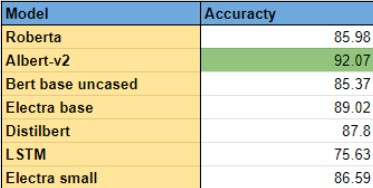
\includegraphics{accuracy.jpg}
\end{center}
\caption[ความแม่นยำในการทำนายของโมเดลแต่ละแบบ]{ความแม่นยำในการทำนายของโมเดลแต่ละแบบ}
\label{fig:ความแม่นยำในการทำนายของโมเดลแต่ละแบบ}
\end{figure}


\section{โปรแกรมอ่านรายงานประจำปีของบริษัท}

\enskip \enskip \enskip เมื่อได้โมเดลที่ดีที่สุดสำหรับการการจำแนกชนิดประโยคซึ่งก็คือ Albert-v2  
เราจึงทดลองนำโมเดลนั้นไปสร้างโปรแกรมสำหรับจำแนกประโยคของรายงานประจำปีทั้งเล่มในทุกๆปีย้อนหลัง5ปีของบริษัทที่ใส่เข้าเป็นอินพุต
โดยเมื่อเราได้ทดลองใช้โปรแกรมนั้นกับหลายๆบริษัทแล้ว จากผลลัพธ์ที่ได้เราจึงได้ข้อมูลที่สรุปได้ว่าบริษัทส่วนมากมักมีแนวโน้มในการพูดถึงประโยคที่เกี่ยวข้องกับสิ่งแวดล้อมและสังคมเพิ่มมากขึ้นทุกปี
ซึ่งอาจเป็นเพราะประเด็นของESGที่กำลังได้รับความนิยมในปัจจุบัน
และประโยคส่วนมากเป็นประโยคที่เกี่ยวข้องกับธรรมาภิบาลและไม่เกี่ยวข้องกับประเด็นไหนเลย
เพราะในรายงานประจำปีมักมีการพูดถึงเรื่องการบริหารจัดการในบริษัทเป็นจำนวนมากและเรื่องอื่นๆที่ไม่เกี่ยวข้องกับประเด็นESGก็มีอยู่มากเช่นกัน

\begin{figure}
\begin{center}
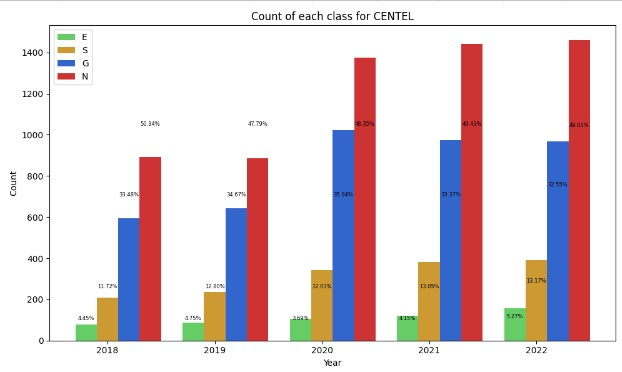
\includegraphics{graph.jpg}
\end{center}
\caption[ทดลองใช่โปรแกรมอ่านรายงานประจำปีของบริษัท CENTEL]{ทดลองใช่โปรแกรมอ่านรายงานประจำปีของบริษัท CENTEL}
\label{fig:ทดลองใช่โปรแกรมอ่านรายงานประจำปีของบริษัท CENTEL}
\end{figure}